\documentclass[12pt]{article}
\usepackage{graphicx} % For including images
\usepackage[margin=1in]{geometry} % For setting page margins
\usepackage{amsmath} % For extended mathematical formatting
\usepackage{fancyhdr} % For custom headers and footers
\usepackage{float} 
\usepackage{subcaption} % Updated to use subcaption instead of subfigure
\setlength{\headheight}{15pt} % Adjust headheight as recommended
\pagestyle{fancy}
\fancyhf{}
\rhead{EE569 Digital Image Processing}
\lhead{HOMEWORK \#1}
\rfoot{Page \thepage}

\begin{document}
	
	\begin{center}
		\Large
		\textbf{Homework \#2}
		
		\vspace{0.2cm}
		\normalsize
		Issued: 01/31/2024 \hfill Due: 02/19/2024
	\end{center}

\section*{Problem 1:Edge Detection}
\subsection*{(a) Sobel Edge Detector}
\begin{figure}[H]
	\centering
	\begin{subfigure}{0.45\textwidth}
		\centering
		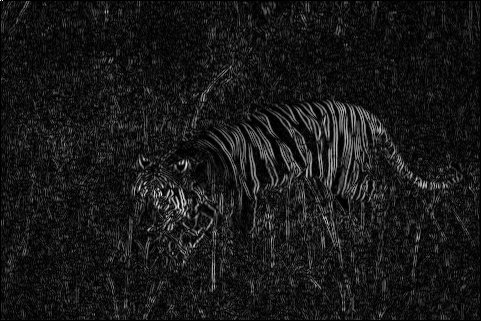
\includegraphics[width=\textwidth]{TigerX.jpg}
		\caption{Tiger X-Gradient}
		\label{fig:tiger.x}
	\end{subfigure}
	\begin{subfigure}{0.45\textwidth}
		\centering
		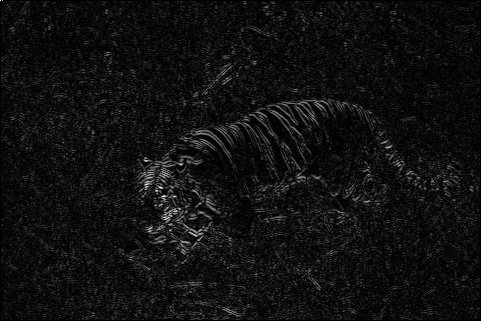
\includegraphics[width=\textwidth]{TigerY.jpg}
		\caption{Tiger Y-Gradient}
		\label{fig:tiger.y}
	\end{subfigure}
	
	\begin{subfigure}{0.45\textwidth}
		\centering
		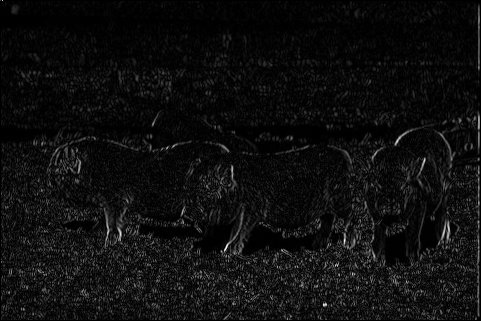
\includegraphics[width=\textwidth]{PigX.jpg}
		\caption{Pig X-Gradient}
		\label{fig:pig.x}
	\end{subfigure}
	\begin{subfigure}{0.45\textwidth}
		\centering
		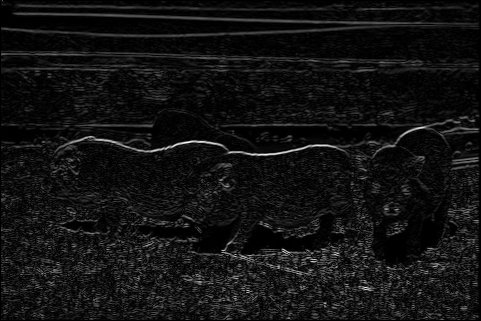
\includegraphics[width=\textwidth]{PigY.jpg}
		\caption{Pig Y-Gradient}
		\label{fig:pig.y}
	\end{subfigure}
	\caption{(1)Normalized Results of X and Y gradients}
	\label{p1a1}
\end{figure}

\begin{figure}[H]
	\centering  %图片全局居中
	\begin{subfigure}{0.45\textwidth}
		\centering
		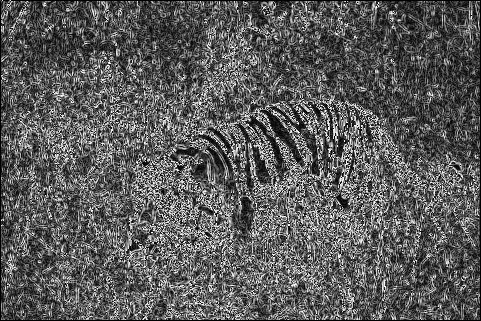
\includegraphics[width=\textwidth]{Tiger1.jpg}
		\caption{Tiger Gradient Magnitude Map}
		\label{tiger.gradien}
	\end{subfigure}
	\begin{subfigure}{0.45\textwidth}
		\centering
		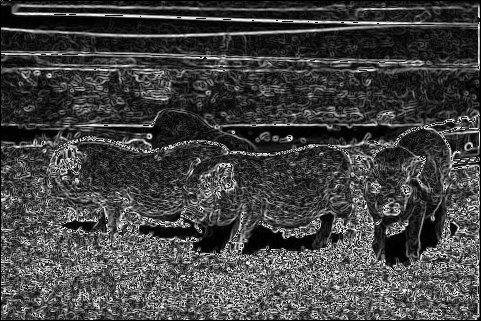
\includegraphics[width=\textwidth]{Pig1.jpg}
		\caption{Pig Gradient Magnitude Map}
		\label{pig.gradient}
	\end{subfigure}
	\caption{(2)Normalized Gradient Magitude Maps}
	\label{p1a2}
\end{figure}

\begin{figure}[H]
	\centering 
	\begin{subfigure}{0.45\textwidth}
		\centering
		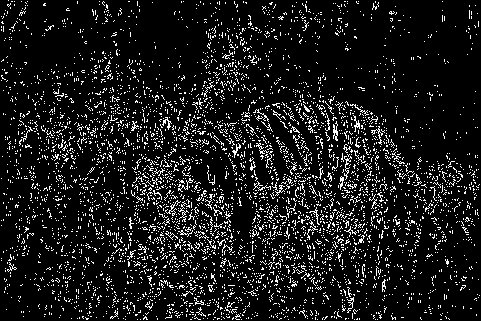
\includegraphics[width=\textwidth]{Tiger90.jpg}
		\caption{Tiger Edge Map with Threshold of 90\%}
		\label{fig:tiger.90}
	\end{subfigure}
	\hfill
	\begin{subfigure}{0.45\textwidth}
		\centering
		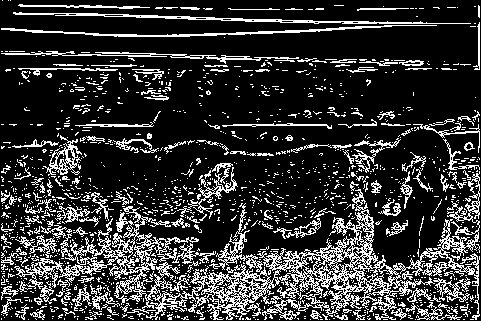
\includegraphics[width=\textwidth]{Pig80.jpg}
		\caption{Pig Edge Map with Threshold of 80\%}
		\label{fig:pig.80}
	\end{subfigure}
	\caption{(3) Edge Maps with Threshold}
	\label{p1a3}
\end{figure}


\subsection*{(b) Canny Edge Detector}
	\begin{itemize}
	\item[(1)] Non-maximum suppression in the Canny edge detector is an approach to find edges. First we search throught all pixels in the image and find those points which are higher than a high threshold, and label them as edges. Then pixels near the determined edges are checked, those higher than a lower threshold are also labeled as edges. 
	
	\item[(2)] High Threshold are used to determine the most significant edges. Low Threshold can determine how much the edges expand.
	
	\item[(3)] Show in Figure with label figuriere \ref*{p1b1} and figuriere \ref*{p1b2}. We can see that when higher high threshold is applied, only more significant pixels with larger gradients will be classified as primary edges, which makes less false positives, but increases the chance of false negative. And when lower high threshold is applied, more points will be classified as primary edge pixels, increasing more environment point that are wrongly classified as edges. And a higher low threshold will decrease how much each edge expand. When similar high thresholds are applied, pictures with higher low threshold will have shorter edges expand from the basic edge points. 

	\end{itemize}

\begin{figure}[H]
	\centering  %图片全局居中
	\begin{subfigure}{0.32\textwidth}
		\centering
		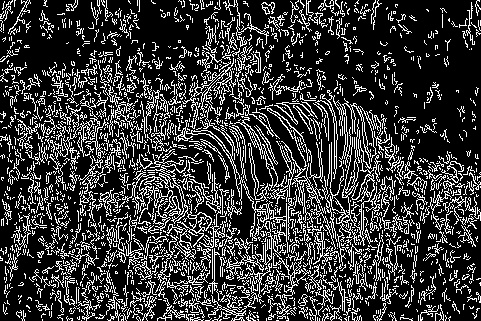
\includegraphics[width=\textwidth]{TigerCanny120_220.jpg}
		\caption{Threshold 120/220}
		\label{fig:tigerCanny.120_220}
	\end{subfigure}
	\hfill
	\begin{subfigure}{0.32\textwidth}
		\centering
		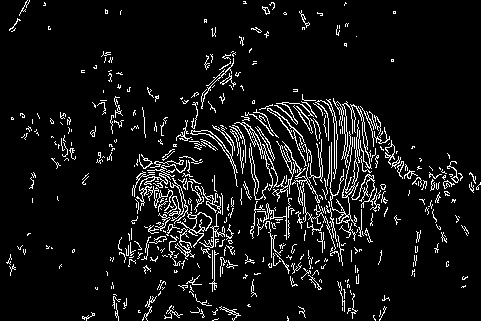
\includegraphics[width=\textwidth]{TigerCanny200_400.jpg}
		\caption{Threshold 200/300}
		\label{fig:tigerCanny.200_400}
	\end{subfigure}
	\hfill
	\begin{subfigure}{0.32\textwidth}
		\centering
		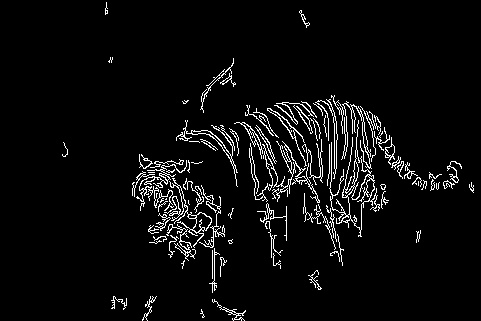
\includegraphics[width=\textwidth]{TigerCanny180_600.jpg}
		\caption{Threshold 180/600}
		\label{fig:tigerCanny.180_600}
	\end{subfigure}
	\caption{Tiger Canny Edge Map}
	\label{p1b1}
\end{figure}

\begin{figure}[H]
	\centering  %图片全局居中
	\begin{subfigure}{0.32\textwidth}
		\centering
		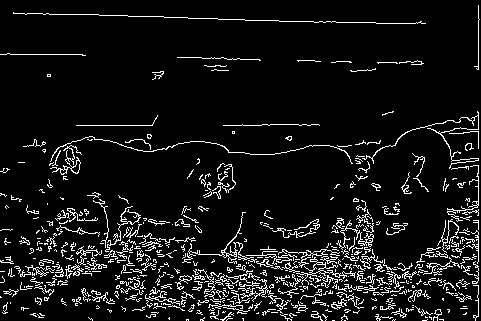
\includegraphics[width=\textwidth]{PigCanny150_300.jpg}
		\caption{Threshold 150/300}
		\label{fig:PigCanny.150_300}
	\end{subfigure}
	\hfill
	\begin{subfigure}{0.32\textwidth}
		\centering
		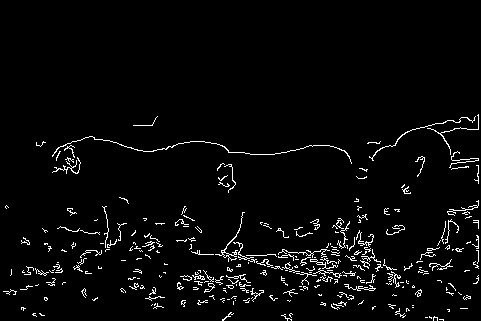
\includegraphics[width=\textwidth]{PigCanny200_400.jpg}
		\caption{Threshold 200/400}
		\label{fig:PigCanny.200_400}
	\end{subfigure}
	\hfill
	\begin{subfigure}{0.32\textwidth}
		\centering
		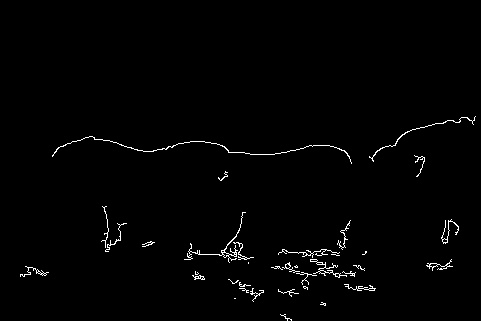
\includegraphics[width=\textwidth]{PigCanny180_600.jpg}
		\caption{Threshold 180/600}
		\label{fig:PigCanny.180_600}
	\end{subfigure}
	\caption{Pig Canny Edge Map}
	\label{p1b2}
\end{figure}


\section*{Problem 2: Digital Half-toning}
\subsection*{(a) Dithering}
\begin{figure}[H]
	\centering 
	\begin{minipage}[b]{0.45\textwidth} 
		\centering
		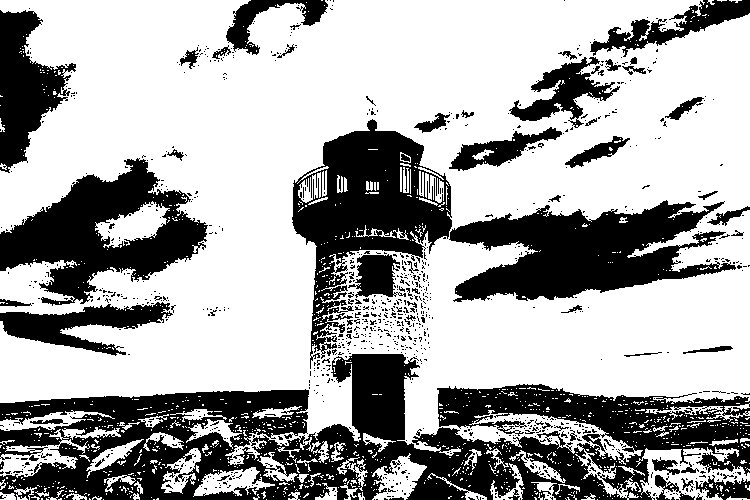
\includegraphics[width=0.8\textwidth]{Lighthouse_fixed}
		\caption{Lighthouse Image with Fixed Thresholding}
		\label{LighthouseFixed}
	\end{minipage}
	\begin{minipage}[b]{0.45\textwidth} 
		\centering 
		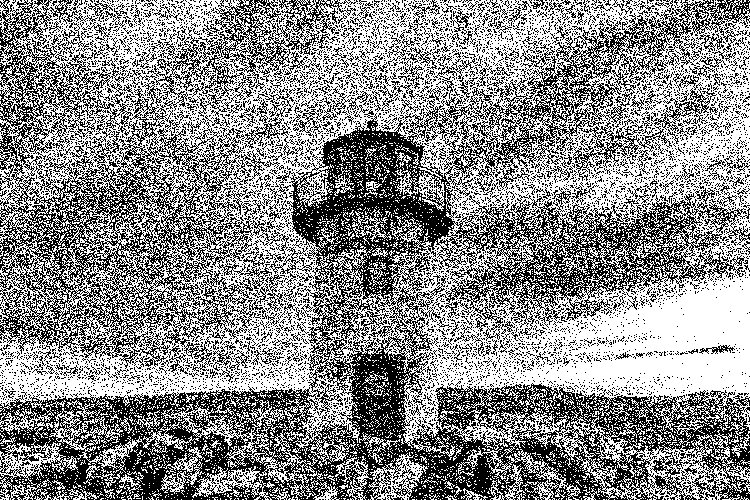
\includegraphics[width=0.8\textwidth]{Lighthouse_random}
		\caption{Lighthouse Image with Random Thresholding}
		\label{LighthouseRandom}
	\end{minipage}
\end{figure}
\begin{figure}[H]
	\centering  %图片全局居中
	\begin{subfigure}{0.32\textwidth}
		\centering
		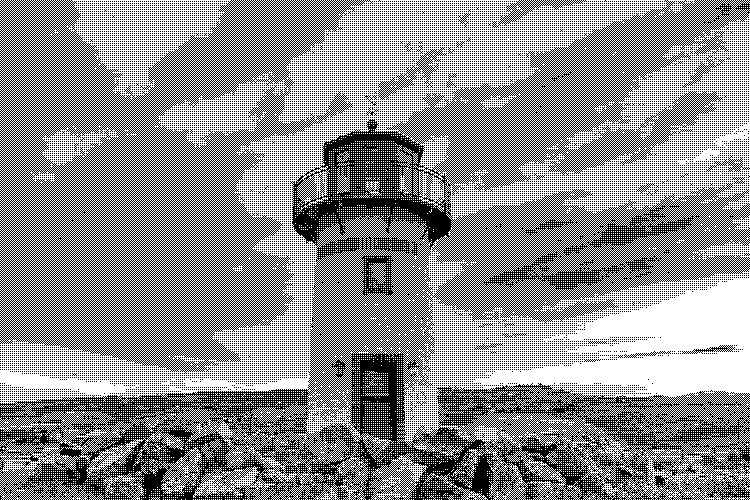
\includegraphics[width=\textwidth]{LighthouseI_2.jpg}
		\caption{Processed Image with $I_2$ Ditering Matrix}
		\label{fig:LighthouseI_2}
	\end{subfigure}
	\hfill
	\begin{subfigure}{0.32\textwidth}
		\centering
		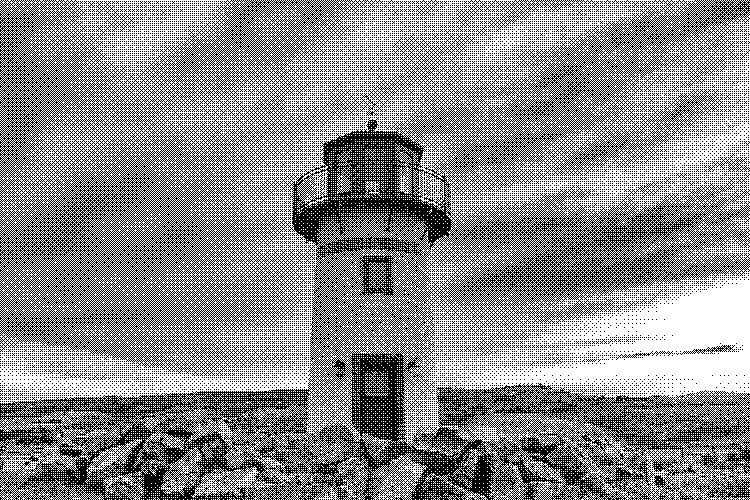
\includegraphics[width=\textwidth]{LighthouseI_8.jpg}
		\caption{Processed Image with $I_8$ Ditering Matrix}
		\label{fig:LighthouseI_8}
	\end{subfigure}
	\hfill
	\begin{subfigure}{0.32\textwidth}
		\centering
		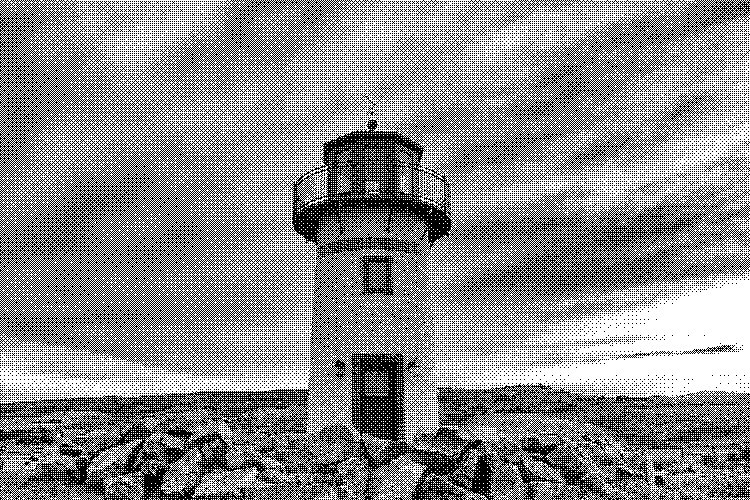
\includegraphics[width=\textwidth]{LighthouseI_32.jpg}
		\caption{Processed Image with $I_32$ Ditering Matrix}
		\label{fig:LighthouseI_32}
	\end{subfigure}
	\caption{Pig Canny Edge Map}
	\label{p2a2}
\end{figure}
(3 )The $I_2$ matrix results in coarse dithering with more pronounced patterns and potential loss of detail. Transitioning to $I_8$ provides smoother halftoning and better detail preservation, suitable for higher resolutions. However, while $I_32$ can provide better halftone quality than $I_8$,  in the case of Lighthouse.raw, the improvement becomes less noticeable.

\subsection*{(b) Error Diffusion}
\begin{figure}[H]
	\centering  %图片全局居中
	\begin{subfigure}{0.4\textwidth}
		\centering
		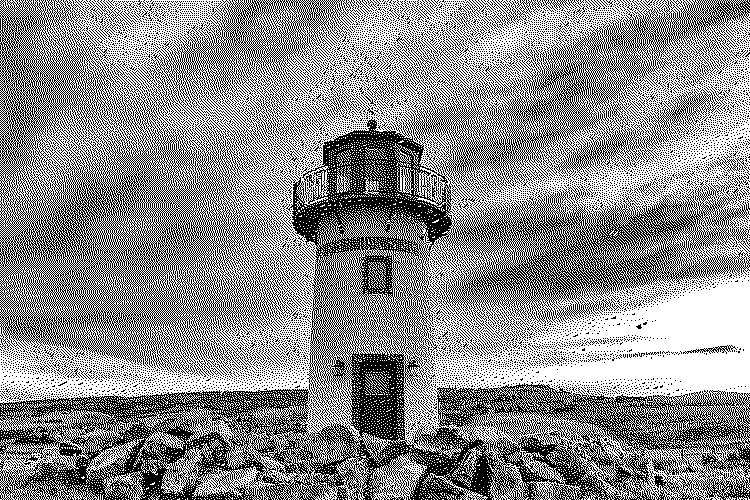
\includegraphics[width=\textwidth]{Lighthouse_floyd.jpg}
		\caption{Processed Image with Floyd-Steinberg’s error diffusion}
		\label{fig:Lighthouse_floyd}
	\end{subfigure}
	\hfill
	\begin{subfigure}{0.4\textwidth}
		\centering
		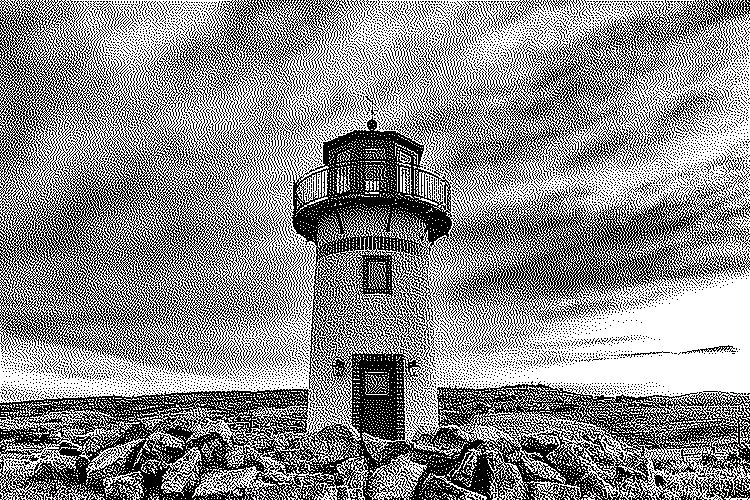
\includegraphics[width=\textwidth]{Lighthouse_JIN.jpg}
		\caption{Processed Image with Jarvis, Judice, and Ninke (JJN)}
		\label{fig:Lighthouse_JIN}
	\end{subfigure}
	\hfill
	\begin{subfigure}{0.4\textwidth}
		\centering
		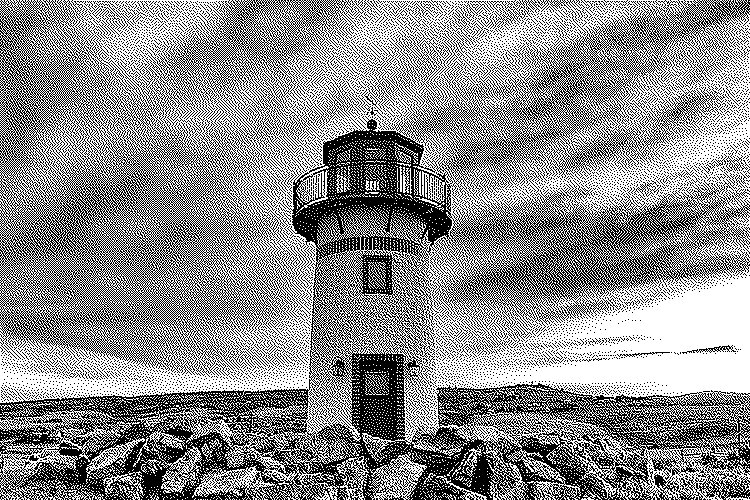
\includegraphics[width=\textwidth]{Lighthouse_Stucki.jpg}
		\caption{Processed Image with Error diffusion proposed by Stucki}
		\label{fig:Lighthouse_Stucki}
	\end{subfigure}
	\caption{Error Diffusion with three different Matrix Methods}
	\label{p2a3}
\end{figure}
In this case, I prefer the method of stucki and JJN, which keeps most details of the original image, and with almost no noise. The method of floyd keeps also good details but brings a little random noises to the image. The fixed thresholding method lost lots of details, and the random thresholding method brings severe salt\&pepper noises. And Dithering Matrix's result is not as good as error diffusion in terms of contrasts and other details. \\

I have an idea of pre-processing local enhancement processing, such as edge enhancement and contrast amplification, should be applied to highlight main features before employing the error diffusion technique. This approach would prevent the loss of details and minimize noise introduction. Additionally, further processing of the halftoned image post error diffusion, like applying median filtering, could remove isolated noise points. For instance, the Floyd method may generate isolated noise which can be mitigated with this technique.\\\\

(4) Raster scanning processes an image line by line from one side to the other, makes the processed image with unnatural strips in horizonal direction, which is called directional artifacts. While serpentine scanning alternates direction every line, reducing such artifacts and evenly distributing errors for a more consistent image quality.

\section*{Problem 3: Color Half-toning with Error Diffusion}
\subsection*{(a) Separable Error Diffusion}
\begin{figure}[H]
	\centering
	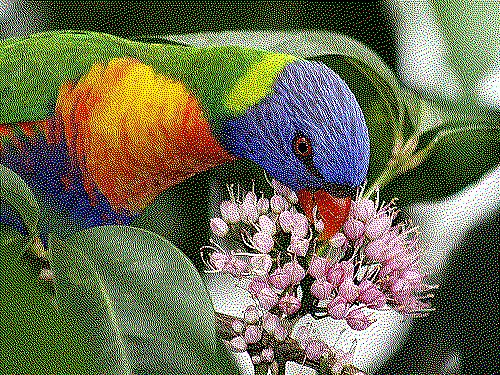
\includegraphics[width=0.7\textwidth]{Bird_seperable.jpg}
	\caption{half-toned color Bird image with Separable Error Diffusion}
	\label{fig:Bird_seperable}
\end{figure}
The most significant issue with this image is random noises. The combination of the 8 colors cannot form good enough natural colors for human's eyes.  
\subsection*{(b) MBVQ-based Error diffusion} 
\begin{itemize}
	\item[(1)] The key idea of the MBVQ is that instead of directly using comination of 8 color channels, it uses a method that could sharply decrease the existance of K/W, which are on the two ends of brightness diagram.  It turns each pair of K/W with other colors into closer color pairs in the brightness diagram. For example, K-W into M-G, K-Y into R-G, K-C into B-G, K-M into B-R, vise versa for pairs containing W. This could make colors more precisely in human eyes, since human vision is more sensible to brightness than color. Less combination of color pixels with high changes in brightness could decrease the number of noises and unnatural pixels, making the image more natural and with more saturation. 
	
	\item[(2)] I met a wired problem that I could not find where it is.
\end{itemize}
\begin{figure}[H]
	\centering
	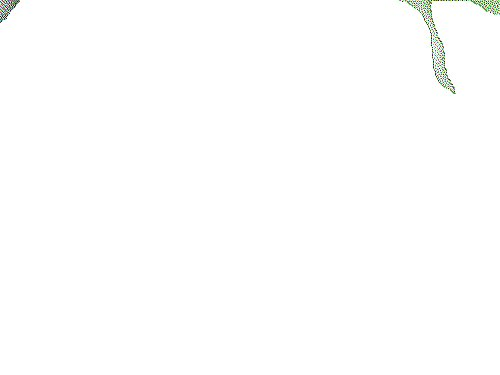
\includegraphics[width=0.7\textwidth]{BirdMBVQ.jpg}
	\caption{half-toned color Bird image with MBVQ Diffusion}
	\label{fig:Bird_MBVQ}
\end{figure}
\end{document}